\chapter{Proyecto de transferencia}

\section{Introducción}

ILa implementación del uso de robots como herramientas pedagógicas para la enseñanza de lenguajes de programación implica una serie de compromisos técnicos y logísticos específicos, desde la adquisición de herramientas para la fabricación y mantenimiento de los mismos, hasta la capacitación de los docentes para poder trabajar en el aula.

Dado que un robot es un componente físico, y por lo tanto tiene un coste de adquisición y mantenimiento que puede ser elevado, las decisiones de costo/beneficio son fundamentales -aunque no exclusivas- a la hora de optar utilizar la robótica en un colegio.

Este proyecto de transferencia busca generar la documentación necesaria para que las escuelas técnicas con orientación a la informática o electrónica puedan adoptar e implementar el proyecto de robótica educativa ICARO, poniendo énfasis en la capacitación de docentes y discentes para fabricar el hardware y usarlo en enseñanza de lenguajes de programación.


\section{Justificación}

La implementación de un proyecto de hardware libre, requiere capacitación  especifica en el uso de herramientas de diseño CAD/CAM libres \citep{bareno2011metodologia}, además de una migración de los laboratorios informáticos de la institución, para que puedan trabajar con sistemas operativos GNU/Linux (el sistema propuesto para este proyecto de transferencia).

Los proyectos de hardware libre buscan permitir a las instituciones, usuarios finales y hasta empresas independizarse de un proveedor especifico de tecnología \citep{gonzalez_hardware_2003}. De esa manera las instituciones escolares pueden optimizar su presupuesto en función de las necesidades especificas de cada instituto.

El proyecto pretende transferir efctivamente el ''saber como'' (Know-how), para que la institución participante pueda re diseñar, fabricar e implementar placas NP07 del proyecto ICARO, contemplando desde la obtención y compra de los elementos de fabricación, hasta su implementación en el aula, así como la adecuación del laboratorio informático para el trabajo con el hardware propuesto.
 
\section{objetivos}
\subsection*{generales}
\begin{enumerate}
  \item Promover el uso de software y hardware libre en los colegios técnicos.
  \item Transferir el conocimiento para implementar la fabricación de hardware del proyecto ICARO en la institución participante.
  \item Abaratar costos para la institución por el uso de licencias libres.
  \item capacitar a los docentes en la enseñanza de lenguajes de programación.
\end{enumerate}
\subsection*{especificas}
\begin{enumerate}
  \item Preparar un espacio de la institución como laboratorio de electrónica.
  \item Capacitar a docentes en la construcción del hardware propuesto.
  \item Capacitar a los docentes en el uso de la propuesta curricular para el hardware NP07.
\end{enumerate}

\section{licencias}
Todas la documentación del proyecto (código fuente, planos esquemáticos del hardware y documentación pedagógica) esta distribuida con las licencias del proyecto GNU\footnote{https://fsf.org/es}  o de la fundación \textit{creative commons}\footnote{http://creativecommons.org.ar/}, la elección de una u otra forma de licenciamiento esta determinado de la siguiente forma \citep{bareno2011metodologia}:
\begin{itemize}
  \item En el caso de todo el  código fuente (python o C), planos esquemáticos del hardware y planos del pcb, sera distribuido con la licencia GNU/GPL V3\footnote{https://lslspanish.github.io/translation\_GPLv3\_to\_spanish/} \footnote{https://www.gnu.org/licenses/gpl\-3.0.en.html}.
  \item Para toda la documentación que no sea referida a los temas anteriores (documentación técnica) sera distribuida con el formato de licenciamiento de la fundación \textit{creative commons}, usando el formato de licencia '' Reconocimiento – Compartir Igual (by-sa)\footnote{http://creativecommons.org.ar/licencias}''.  Licencia que permite el uso comercial del proyecto y de las posibles obras derivadas del mismo, teniendo en cuenta que la distribución de las cuales se debe hacer con una licencia igual a la que regula la obra original del proyecto.
\end{itemize}

\section{metodologia}

La metodología propuesta para el proyecto de transferencia se basa en tres etapas, una primera instancia donde se acondicionara la institución para poder implementar la fabricación del hardware para luego en la segunda etapa, capacitar a los docentes en la fabricación y mantenimiento de las placas NP07. La tercera etapa es la implementación dentro del aula

Luego de la primera instancia de presupuesto y adquisición de materiales, se procederá a impartir el curso de capacitación y acompañamiento a los docentes participantes del proyecto, donde se acondicionara un espacio de la institución para funcionar como laboratorio de desarrollo electrónico, ademas de taller para la fabricación del hardware del proyecto (las placas NP07). Durante la primera mitad del curso, los participantes se instruirán en el uso de alternativas libres para el desarrollo de PCBs mediante el uso de software CAD/CAM KICAD, así mismo se tomara contacto con cada modulo de fabricación del hardware poniendo el énfasis en el puntos de comprobación y reparación. La idea de este primer encuentro es poder comprender el funcionamiento y construcción de las placas.

La segunda mitad del curso de capacitación esta destinada a el desarrollo de las secuencias didácticas especificas que los docentes darán en los cursos de lenguajes de programación, usando el hardware NP07 como herramienta para el desarrollo de las competencias especificas de las ciencias de la computación \citep{sadosky2013cc}.

\begin{wrapfigure}{R}{0.5\textwidth}
  \begin{center}
    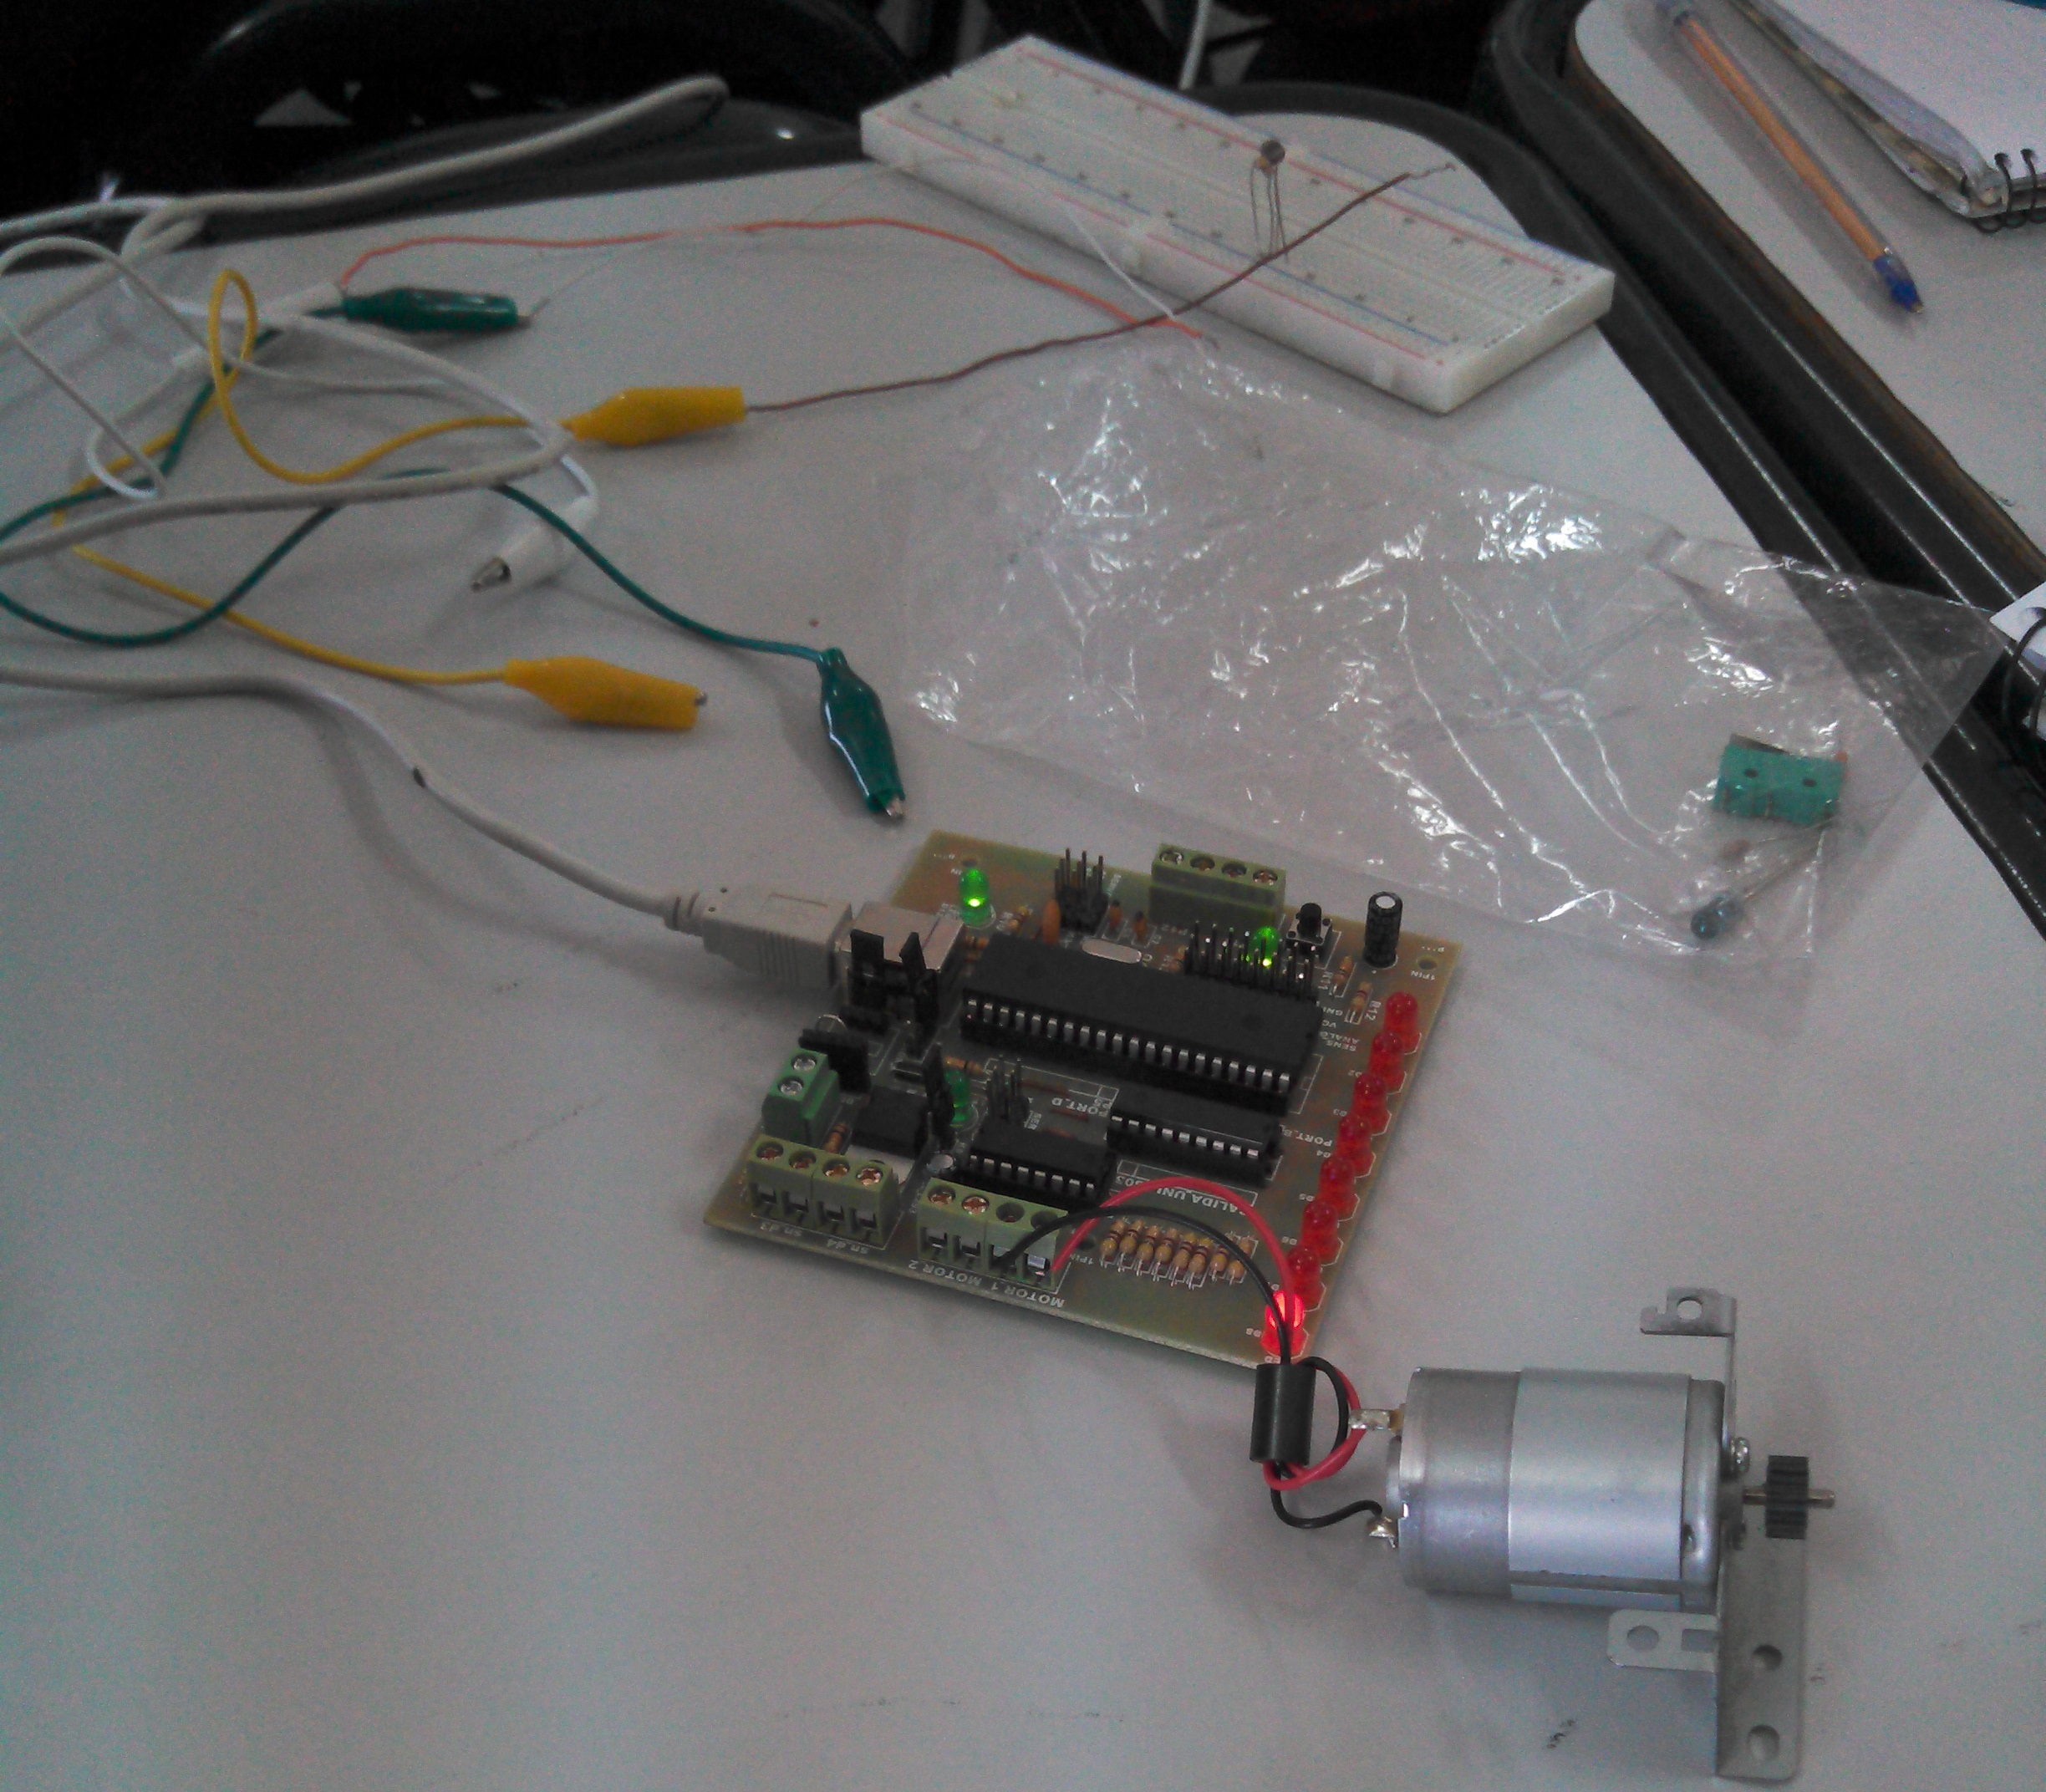
\includegraphics[width=0.5\textwidth]{figuras/np07.jpg}
    \caption[Caption for LOF]{placa para robotica educativa NP07}
    
    \label{fig:placa_np07}
  \end{center}
\end{wrapfigure}

La tercer instancia sera el seguimiento y ayuda de los docentes por parte del equipo de transferencia durante el dictado del curso de enseñanza del lenguaje de programación PYTHON a los discentes de la institución. El dictado de este curso dependerá de cada institución, si deciden ponerlo dentro de un espacio curricular o extra curricular, pero la metodología en ambos casos se basara en la construcción y programación de un robot usando componentes reciclados de equipos de electrónica (impresoras, scanners, equipos reproductores de música).

Al final del curso, los docentes y dicentes podrán generar un documento de retro alimentación con sugerencias para mejorar el desarrollo del proyecto de transferencia tecnológica educativa y que pueda servir para futuras implementaciones en otras instituciones.

\section{Capacitación}

El esquema de capacitación esta elaborado en los anexos 1, 2 y 3, donde el anexo 1 es el esquema de armado del hardware NP07 (guiá de construcción) diseñada por la comunidad de usuarios y desarrolladores de ICARO, el anexo 2 es la capacitación para la construcción del hardware NP07 para docentes y el anexo 3 son las secuencias didácticas diseñadas para trabajar con los discentes durante el segundo cuatrimestre.

Las clases serán programadas para ser cursadas 1 ves a la semana, durante el horario escolar, o en horario extra escolar, en función de la elección de la institución con respecto a la cursada.

\section{duración}

La duración del proyecto sera de 1 año escolar, donde el primer cuatrimestre escolar se tomara para el presupuestado de componentes y la capacitación docente para, luego en el segundo cuatrimestre, pasar al curso de enseñanza de programación con robots para los discentes de la institución.

Terminado el proyecto, la institución educativa contara con el apoyo de la comunidad de desarrollo de ICARO a través de los canales habituales para consultas y recomendaciones que se manejan en los proyectos de desarrollo de software libre (Salas de chat IRC, listas de correo y foros).

\section{gantt}

El diagrama de gantt propuesto, contempla un proceso de un año de trabajo dentro de la institución escolar que participara de el proyecto de transferencia tecnológico educativo, donde el primer cuatrimestre de año escolar se utilizara para poder capacitar a los docentes y preparar las instalaciones para poder impartir un curso inicial de robótica con los discentes. Al final del año escolar, los discentes podrán mostrar un trabajo final usando el hardware propuesto.

El diagrama esta propuesto para tener seis instancias de intervención:

\begin{enumerate}
  \item \textbf{Análisis y evaluación de la institución}: En esta etapa, se determinara las necesidades del colegio, las características y estado de las instalaciones y en que etapa de la formación escolar se implementara la curricula de enseñanza de programación (tomando como referencia las practicas educativas que se vengan implementando en la escuela).
  \item \textbf{Presupuesto:} Teniendo en cuenta las posibilidades económicas de la institución, se tomara las decisiones presupuestarias de equipamiento para el laboratorio y la adquisición de componentes y herramientas para la fabricación de las placas NP07 del proyecto ICARO. En esta etapa se buscaran los proveedores zonales para componentes electrónicos 
  \item \textbf{Compra de componentes:} Aprobado el prepuesto, se procederá a comprar todas las herramientas y componentes necesarios para poder acondicionar la instalación destinada a alojar el laboratorio de desarrollo.
  \item \textbf{Capacitación docente:} Con las instalaciones preparadas y acondicionadas, se trabajara con los docentes seleccionados en un curso de capacitación de dos meses de duración  y cursada semanal (ocho clases en total). La idea principal es que los mismo docentes puedan fabricar las primeras placas NP07 para poder luego enseñarle a sus discentes como hacerlo, aprendiendo las características técnicas del hardware y el software de trabajo.
  \item \textbf{Curso para los discentes de la institución:} Terminado el primer cuatrimestre, se implementara el curso de programación  para los discentes seleccionados previamente, con la idea de poder trabajar con los conceptos básicos de las ciencias de la computación, a través del diseño y desarrollo de un robot educativo y la programación mediante lenguaje PYTHON del mismo.
  \item \textbf{Trabajo final de los discentes:} En esta etapa, los discentes que participaron del curso, trabajaran en un proyecto de final de curso, donde diseñaran un robot y lo podran exponer en una feria de ciencia escolar que prepare la institución. Esta etapa se utilizara como parte de una auto evaluación del proyecto, para poder darle seguimiento el año siguiente y poder ''pulir'' falencias y proponer mejoras.   
\end{enumerate}

La finalidad del proyecto es lograr que en un año escolar, la institución pueda estar preparada para fabricar, reparar y mantener el hardware de el proyecto ICARO, para luego poder utilizarlo como herramienta pedagógica para los cursos de enseñanza de lenguajes de programación.

\begin{figure}[H]
  \begin{center}
    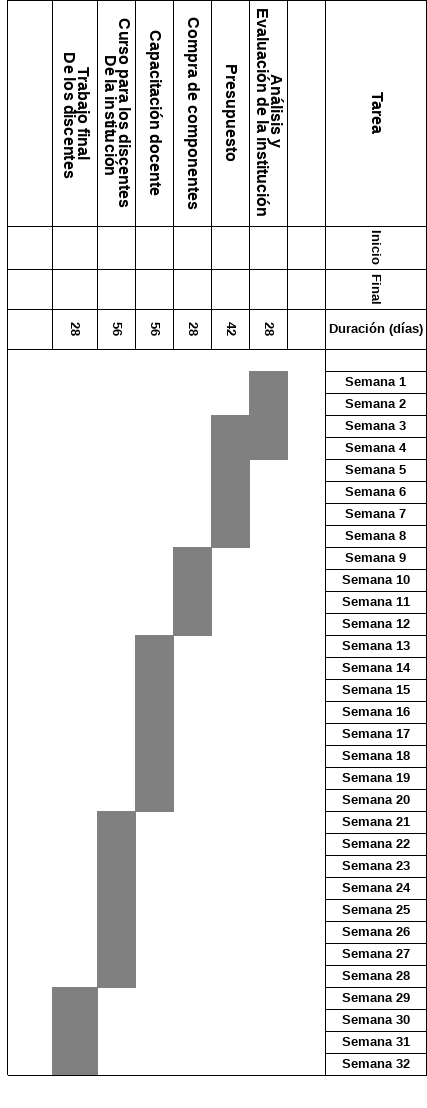
\includegraphics[width=0.5\textwidth]{./figuras/gantt2.png}
    \caption{diagrama de gantt}
    \label{fig:gantt}
  \end{center}
\end{figure}


\section{requerimientos para el laboratorio de desarrollo}
Para poder montar un laboratorio de desarrollo electrónico, la institución participante deberá acondicionar un espacio con las siguientes características:

\begin{itemize}
  \item Mesas de trabajo amplias para poder disponer del equipamiento.
  \item Zapatillas eléctricas para disponer de los soldadores de estaño.
  \item Pizarrón y pantalla para proyector.
  \item Laboratorio de Computadoras (pueden ser Pcs de escritorio o notebooks) preparadas con sistema GNU/Linux.
  \item mueble tipo placar con cerradura, para almacenar las herramientas y componentes electrónicos. 
\end{itemize}

En función de la cantidad de participantes que se determine en la etapa de evaluación y el presupuesto aprobado, se tendrán en cuenta las dimensiones de necesarias para el laboratorio así como las cantidades necesarias de los elementos requeridos para el desarrollo del proyecto. Como referencia se debe tener en cuenta que que para poder trabajar en el laboratorio, los discentes deberán formar grupos de entre 3 y 5 integrantes. 

\section{herramientas}

Las herramientas necesarias para la fabricación del las placas NP07 se pueden dividir en 3 tipos: 

\begin{enumerate}
  \item Herramientas especificas del laboratorio y que solo es necesario adquirir una para el laboratorio.
  \item Herramientas para la fabricación de las placas NP07 y que se repartirán en formato ''kit'' por cada grupo de trabajo.
  \item Herramientas generales para el diseño de un robot y trabajo en el aula.
\end{enumerate}

Las herramientas especificas del laboratorio son todas las que permiten el trabajo dentro del mismo, pero que no forman parte especifica del armado del hardware y que pueden ser adquiridas en pequeñas cantidades, siendo herramientas auxiliares para la tarea. Los requerimientos de estas herramientas son:

\begin{itemize}
  \item Equipo proyector de video.
  \item Programador electrónico para micro controladores PICs de la firma Microchip\textregistered.
  \item Juego de destornilladores para electrónica.
  \item Mini torno con set de mechas y accesorios.
  \item Perforadora de mano.
  \item Perforadora de banco.
  \item Impresora láser mono cromática.
  \item Plancha de mano (para la fabricación de PCBs caseros).
\end{itemize}

Algunas herramientas opcionales, que por su excesivo precio no son incluidas entre las requeridas:

\begin{itemize}
  \item Impresora 3D.
  \item Osciloscopio digital de dos canales.
  \item Mini Fresadora CNC (Control numérico por computadora) para circuitos electrónicos.
  \item Perforadora de banco. 
\end{itemize}

En el caso de las herramientas que se usaran para la fabricación de las placas NP07, se necesita comprar el siguiente Kit de herramientas básicas para soldadura con estaño. En función de la cantidad de participantes (si el curso de fabricación se hará extensivo a docentes y discentes) es recomendable comprar un Kit por cada 4 participantes, seria ideal adquirir entre 5 y 10 Kits de soldadura.

Los componentes del kit para soldadura son:

\begin{itemize}
  \item Soldador de estaño tipo cautin de punta cerámica y 40W de potencia.
  \item Protoboard doble de 1360 puntos con terminales de alimentación y base metálica.
  \item Alicate de corte.
  \item Pinza de punta.
  \item De-soldador a pistón.
  \item Soporte multi propósito con lupa.
  \item Cinta malla de-soldante 1,5 Mts.
  \item Soporte soldador con esponja de limpieza.
  \item 1,5 Mts Estaño 60/40 0,8mm con fundente.
  \item Multimetro digital.
\end{itemize}

Las herramientas generales necesarias, sera usadas para fabricar robots, dar mantenimiento al equipamiento adquirido y para reciclar o re utilizar componentes electro-mecanicos que puedan aprovecharse del descarte de componentes en desuso que la institución consiga. Las herramientas basicas son:

  \begin{itemize}
    \item Set de destornilladores relojeros.
    \item Pinzas.
    \item Tijeras de cartón.
    \item Pistola encoladora de silicona.
    \item Cúter (trincheta).
    \item reglas metálicas.
  \end{itemize}
  
\section{laboratorio informatico}

Teniendo en cuenta que el uso del robots esta planeado como un sistema auxiliar para la enseñanza de programación en los discentes, la instalación de un laboratorio informático deberá contar con las siguientes características a nivel de software:

\begin{itemize}
  \item Sistema GNU/ Linux instalado (Fedora o Huayra linux).
  \item Entorno gráfico XFCE (recomendado por su poco consumo de memoria RAM).
  \item Interprete python 2.7 y python 3.0.
  \item Consola interactiva para python (IPYTHON).
  \item Entorno de desarrollo integrado (IDE) para python (GEANY).
  \item Software de desarrollo electronico (KICAD).
  \item Software de diseño 3d (BLENDER Y FreeCad).
  \item Software de diseño vectorial e imágenes (Gimp, INKSCAPE).
  \item Software de control del hardware (ICARO).
  \item Software para cargar bootloaders (PK2CMD).
  \item Editor de texto (LibreOffice).
  \item Librerías para tratamiento de imágenes con python (OPEN-CV).
\end{itemize}

EL laboratorio, al igual que con el kit de herramientas de soldadura, se recomienda que haya por lo menos 1 computadora cada 4 o 5 discentes. Con respecto a la instalación del sistema GNU/Linux, se pueden tomar 3 opciones:

\begin{enumerate}
  \item Formatear las computadoras y solo instalar GNU/Linux (single boot).
  \item Instalar GNU/Linux en una partición del disco, conservando el sistema operativo anterior (dual Boot).
  \item Tener pen drives preparados con GNU/Linux y arrancar el sistema operativo desde el pen drive cada ves que se necesite usar la maquina (sistema LiveUsb Linux).
\end{enumerate}

En función de las necesidades del colegio y de las especificaciones del laboratorio informático, se deberá tomar una de las 3 opciones disponibles.


 
